\documentclass[./Research.tex]{subfiles}

\begin{document}

\def\layersep{2.5cm}

	When constructing Neural Networks, we generally consider the order of inputs to neurons or the order of inputs in a layer, to be irrelivent. However, there is no reason that the order of inputs should be self-evident, and in many cases, the best order of inputs may not be known at all. To examine this, let us create a simple model for a single neuron, where it accepts any number of inputs and has a single output which is the result of applying the 'eval' function to the inputs. \\

%diagram of the neuron
\begin{center}
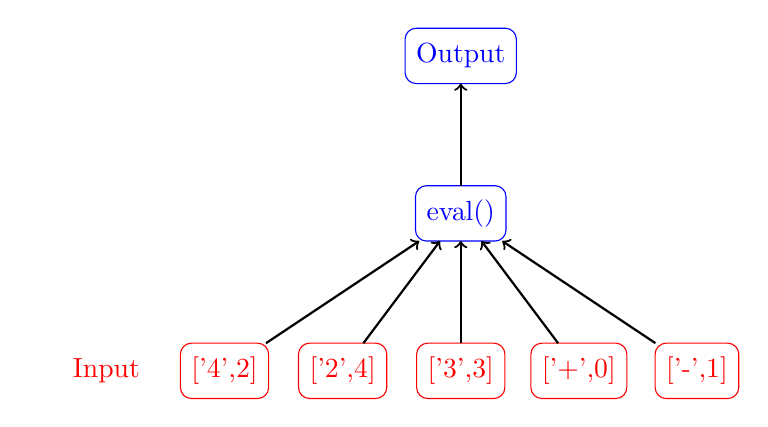
\begin{tikzpicture}

\tikzstyle{bordered} = [shape=rectangle, rounded corners, draw, outer sep=0,inner sep=4,minimum size=20]
\tikzstyle{con} = [thick,->]
\tikzstyle{message} = [shape=rectangle, thick, minimum width=2cm]


\node [bordered,red] (v1) at (1,7.5) {['4',2]};
\node [bordered,red] (v5) at (5.5,7.5) {['+',0]};
\node [bordered,red] (v4) at (4,7.5) {['3',3]};
\node [bordered,red] (v3) at (2.5,7.5) {['2',4]};
\node [bordered,red] (v6) at (7,7.5) {['-',1]};
\node [bordered,blue] (v2) at (4,9.5) {eval()};
\node [bordered,blue] (v7) at (4,11.5) {Output};

\draw [con] (v1) edge (v2);
\draw [con] (v3) edge (v2);
\draw [con] (v4) edge (v2);
\draw [con] (v5) edge (v2);
\draw [con] (v6) edge (v2);
\draw [con] (v2) edge (v7);


\node [message,red] at (-0.5,7.5) {Input};

\end{tikzpicture} \\
\end{center}
	
	Each input is a tuple where the first index is either an operator or operand, and the second index contains the input's position in the eval function. When the neuron's value is evaluated, all inputs are positioned according to their second index's value. If the tuples in the above diagram were passed into the neuron, it would result in 'eval(+ - 4 3 2)', or simply '3'. \\
	
\textbf{What if we don't know the correct position for the operator and operands?} \\
	Typically, the order of inputs into a neural network isn't given much consideration, particularly when tuning the neurons to a yield a desired result. In this section, we will design a simple algorithm to tune the second index of each input tuple (the index which represents the input's position in eval()) using only the unordered inputs and a few output examples given the inputs. \\

	Let's examine the above diagram, but eliminate all information which requires us to 
know the order of inputs, aside from the output:

%diagram of the neuron
\begin{center}
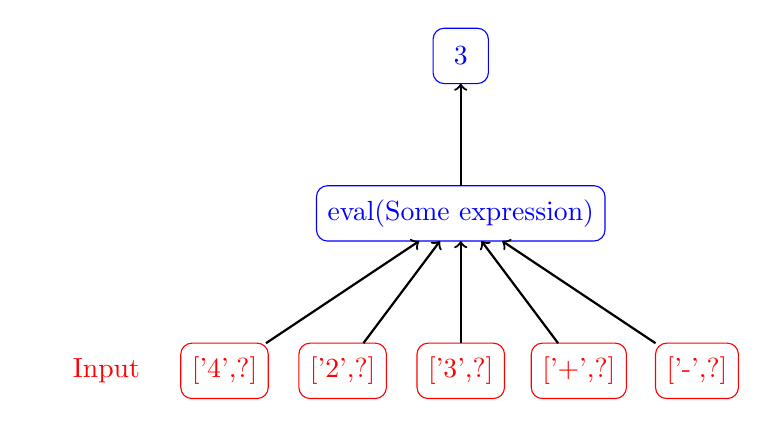
\begin{tikzpicture}

\tikzstyle{bordered} = [shape=rectangle, rounded corners, draw, outer sep=0,inner sep=4,minimum size=20]
\tikzstyle{con} = [thick,->]
\tikzstyle{message} = [shape=rectangle, thick, minimum width=2cm]


\node [bordered,red] (v1) at (1,7.5) {['4',?]};
\node [bordered,red] (v5) at (5.5,7.5) {['+',?]};
\node [bordered,red] (v4) at (4,7.5) {['3',?]};
\node [bordered,red] (v3) at (2.5,7.5) {['2',?]};
\node [bordered,red] (v6) at (7,7.5) {['-',?]};
\node [bordered,blue] (v2) at (4,9.5) {eval(Some expression)};
\node [bordered,blue] (v7) at (4,11.5) {3};

\draw [con] (v1) edge (v2);
\draw [con] (v3) edge (v2);
\draw [con] (v4) edge (v2);
\draw [con] (v5) edge (v2);
\draw [con] (v6) edge (v2);
\draw [con] (v2) edge (v7);


\node [message,red] at (-0.5,7.5) {Input};

\end{tikzpicture} \\
\end{center}

\end{document}
